\documentclass{beamer}

\usetheme{default}
%\usetheme{AnnArbor}
\usecolortheme{beaver}
\setbeamertemplate{navigation symbols}{}
\setbeamertemplate{footline}[frame number]

\usepackage{graphicx}

% Customize section page
\setbeamertemplate{section page}
{
	\begin{centering}
		\begin{beamercolorbox}[sep=12pt,center]{part title}
			\usebeamerfont{section title}\insertsection\par
		\end{beamercolorbox}
	\end{centering}
}

\title{DStauffman Library}
\author{David C. Stauffer}
\date{16 August 2016}

\begin{document}

\begin{frame}
\titlepage
\end{frame}

\section{Agenda}
\begin{frame}
	\frametitle{Agenda}
    \begin{itemize}
        \item DStauffman overview
        \item Tic Tac Toe game
        \begin{itemize}
            \item Interactive demo?
        \end{itemize}
    \end{itemize}
\end{frame}


\section{Description}
\begin{frame}
	\frametitle{What is the dstauffman library?}
    \begin{itemize}
        \item Python library of useful utilities, plus fun games and apps written by David Stauffer.
        \item Available on GitHub as a public repositiory (\url{https://github.com/DStauffman/dstauffman})
        \item Runs on Python v3.5+
        \item Mainly geared towards numerical analysis, so it requires Matplotlib, NumPy, pandas, PyQt5 and a handful of other libraries
    \end{itemize}
\end{frame}

\begin{frame}
	\frametitle{Library High Level View}
    \begin{itemize}
        \item Includes User's Guide, documents written in \LaTeX\  to continue open source software theme
        \item Code documentation using Sphinx and docstrings
        \item Unit test cases
        \item Main areas of code:
        \begin{itemize}
            \item Generic utilities (folder \& file manipulation, enum metaclasses, frozen class attributes, save \& load decorators, etc.)
            \item Quaternion methods
            \item Image Processing (photo manipulation and renaming/resizing)
            \item Batch Parameter Estimator for minimizing cost evaluation of arbitrary functions
            \item Archery scoresheets and tournament brackets
            \item Games
            \begin{itemize}
                \item Pentago
                \item Tic Tac Toe
                \item Knight board
                \item Brick/Rubik's Cube
                \item Playing Cards and games
            \end{itemize}
        \end{itemize}
    \end{itemize}
\end{frame}

\begin{frame}
	\frametitle{Code Size}
    As of 15 August 2016:
    \begin{itemize}
        \item Number of Files: 135.  Of which, 93 are Python code
        \item Total lines of code $\approx$25K
        \item Of these: 13K executable (52\%), 3K blank lines (13\%), 9K comment lines (35\%)
        \item Unit test cases currently cover 76\% of code base, including some unfinished modules
    \end{itemize}
\end{frame}

\begin{frame}
	\frametitle{Tic Tac Toe}
    Interactive Demo (if we can get it up and running, otherwise see backup charts)
    \begin{figure}
        \centering
        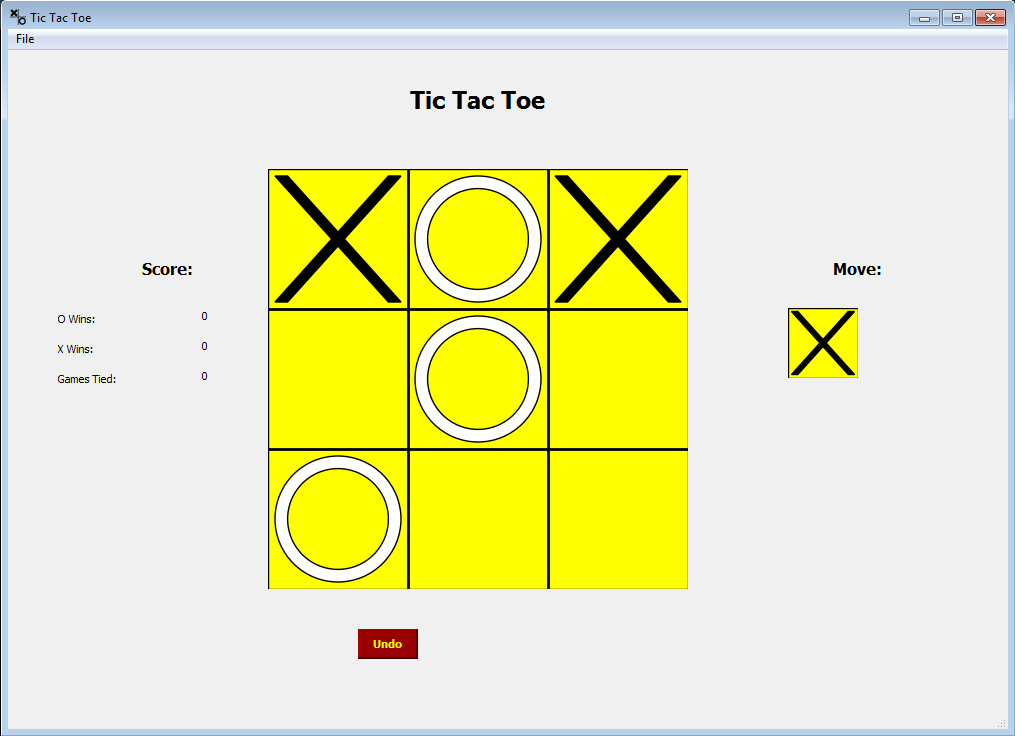
\includegraphics[width=0.8\textwidth]{TicTacToe_Board.png}
    \end{figure}
\end{frame}

\section{Results}
\begin{frame}
	\frametitle{Conclusions}
    The dstauffman library is a fun place to learn and test different Python tricks, while making it a public repository encourages good software practices such as code documentation and unit testing, and hopefully simultaneously provides code that is useful to other people.
\end{frame}

\section{Backup}
\frame{\sectionpage}

\begin{frame}
	\frametitle{Backup Details}
	This project is nice, because it's small enough to wrap your head around it, but makes use of a lot of Python features.  These include:
	\begin{itemize}
		\item numpy arrays for tracking and evaluating board positions.
		\item PyQt5 for the graphics engine with event driven design.
		\item matplotlib plotting capabilities for drawing the board game.
		\item OOP design with classes for capturing game options, current state, and game history, with the ability to save and resume across sessions.  Plus magic methods, like \_\_eq\_\_ and \_\_lt\_\_  to sort the best moves first.
		\item Unit tests and doc tests to demonstrate and verify the functions.
	\end{itemize}
\end{frame}

\begin{frame}
	\frametitle{Backup Details}
	You can play with two players and have the game keep track of the winning history.
	\begin{figure}
		\centering
		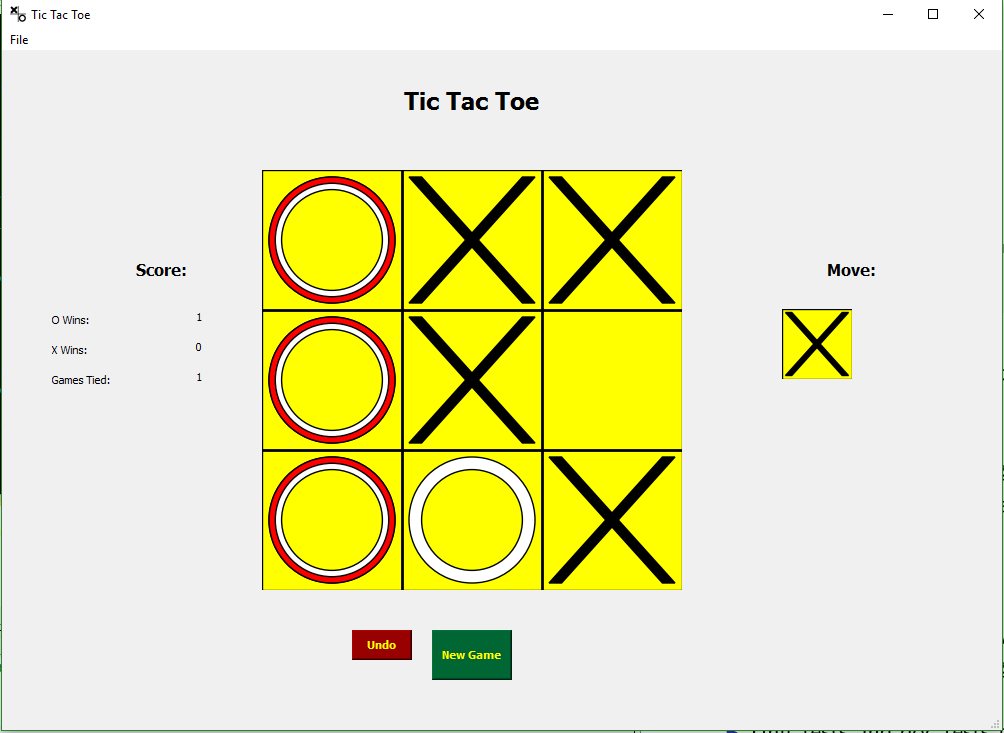
\includegraphics[width=0.8\textwidth]{TicTacToe_Winner.png}
	\end{figure}
\end{frame}

\begin{frame}
	\frametitle{Backup Details}
	Alternatively, you can play against the AI, or even have the computer play against itself.  (If you can beat the computer, I'll buy you lunch).
	\begin{figure}
		\centering
		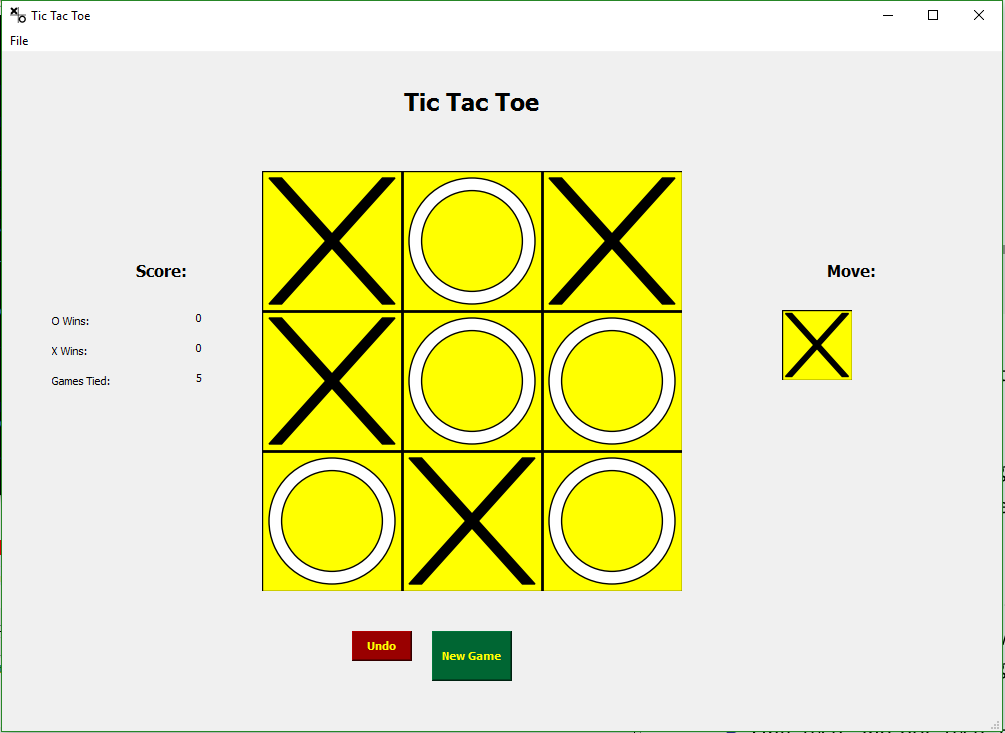
\includegraphics[width=0.8\textwidth]{TicTacToe_Computer_playing_itself.png}
	\end{figure}
\end{frame}

\begin{frame}
	\frametitle{Backup Details}
	You can adjust some options to show how the computer is graded the open squares and where the possible winning moves are.  Relevant controls like ``New Game'' or ``Redo'' appear as necessary.
	\begin{figure}
		\centering
		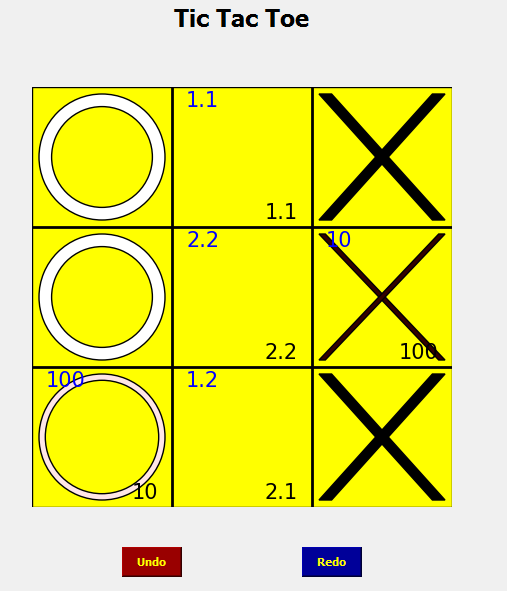
\includegraphics[width=0.4\textwidth]{TicTacToe_Best_moves1.png} \quad%
		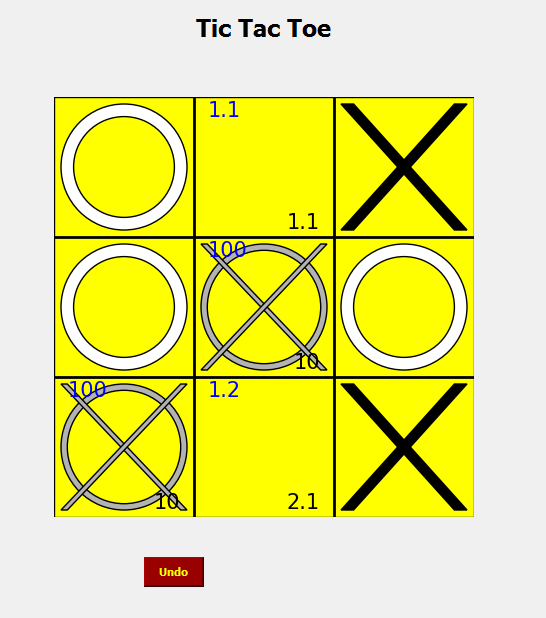
\includegraphics[width=0.4\textwidth]{TicTacToe_Best_moves2.png}
	\end{figure}
\end{frame}

\end{document}
